\section{Classical Robotics}
\label{sec:classical}
\epigraph{\textit{Know your enemy} [...]}{Sun Tzu}

\begin{tldr}
Learning-based approaches to robotics are motivated by the need to (1) generalize across tasks and embodiments (2) reduce dependency on human expertise (3) leverage historical trends on the production of data---all traditionally overlooked by dynamics-based techniques.
\end{tldr}

\subsection{Explicit and Implicit Models}

\begin{figure}
    \centering
    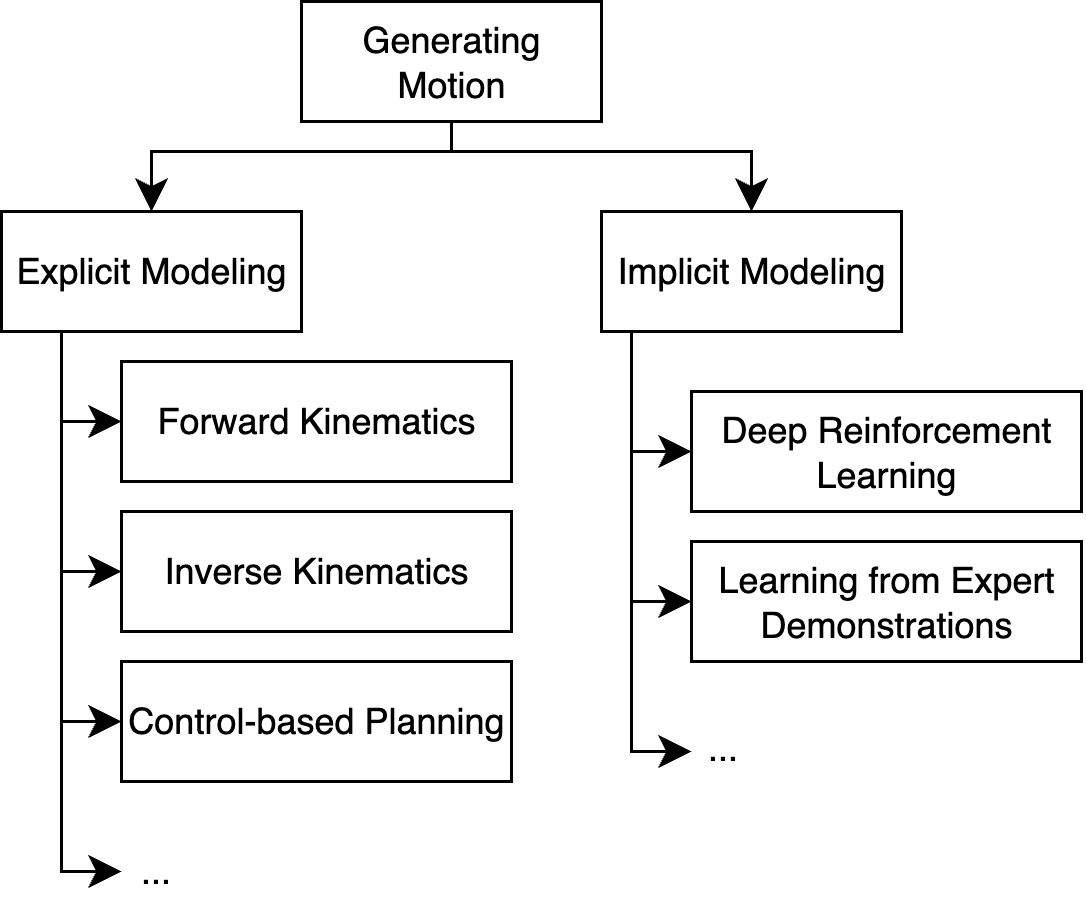
\includegraphics[width=0.5\linewidth]{figures/ch2/ch2-approaches.png}
    \caption{Overview of methods to generate motion (clearly non-exhausitve, see~\citet{bekrisStateRobotMotion2024}). The different methods can be grouped based on whether they explicitly (\emph{dynamics-based}) or implicitly (\emph{learning-based}) model robot-environment interactions.}
    \label{fig:generating-motion-atlas}
\end{figure}

Robotics is concerned with producing artificial motion in the physical world in useful, reliable and safe fashion.
Thus, robotics is an inherently multi-disciplinar domain: producing autonomous motion in the physical world requires, to the very least, interfacing different software (motion planners) and hardware (motion executioners) components.
Further, knowledge of mechanical, electrical, and software engineering, as well as rigid-body mechanics and control theory have therefore proven quintessential in robotics since the field first developed in the 1950s.
More recently, Machine Learning (ML) has also proved effective in robotics, complementing these more traditional disciplines~\citep{connellRobotLearning1993}.
As a direct consequence of its multi-disciplinar nature, robotics has developed as a rather wide array of methods, all concerned with the main purpose of \highlight{producing artificial motion in the physical world}.

Methods to produce robotics motion range from traditional \emph{explicit} models---\highlight{dynamics-based} methods, leveraging precise descriptions of the mechanics of robots' rigid bodies and their interactions with eventual obstacles in the environment---to \emph{implicit} models---\highlight{learning-based} methods, treating artificial motion as a statistical pattern to learn given multiple sensorimotor readings~\citep{agrawalComputationalSensorimotorLearning,bekrisStateRobotMotion2024}.
A variety of methods have been developed between these two extrema.
For instance, ~\citet{hansenTemporalDifferenceLearning2022} show how learning-based systems can benefit from information on the physics of problems, complementing a traditional learning method such as Temporal Difference (TD)-learning~\citet{suttonReinforcementLearningIntroduction2018} with Model-Predictive Control (MPC).
Conversely, as explicit models may be relying on assumptions proving overly simplistic---or even unrealistic---in practice, learning can prove effective to improve modeling of complex phenomena or complement perception~\citep{mccormacSemanticFusionDense3D2016}.
Such examples aim at demonstrating the richness of approaches to robotics, and Figure~\ref{fig:generating-motion-atlas} graphically illustrates some of the most relevant techniques.
Such a list is clearly far from being exhaustive, and we refer to~\citet{bekrisStateRobotMotion2024} for a more comprehensive overview of both general and application-specific methods for motion generation.
In this section, we wish to introduce the inherent benefits of \highlight{learning-based approaches to robotics}---the core focus on this tutorial.

\subsection{Different Types of Motion}

\begin{figure}
    \centering
    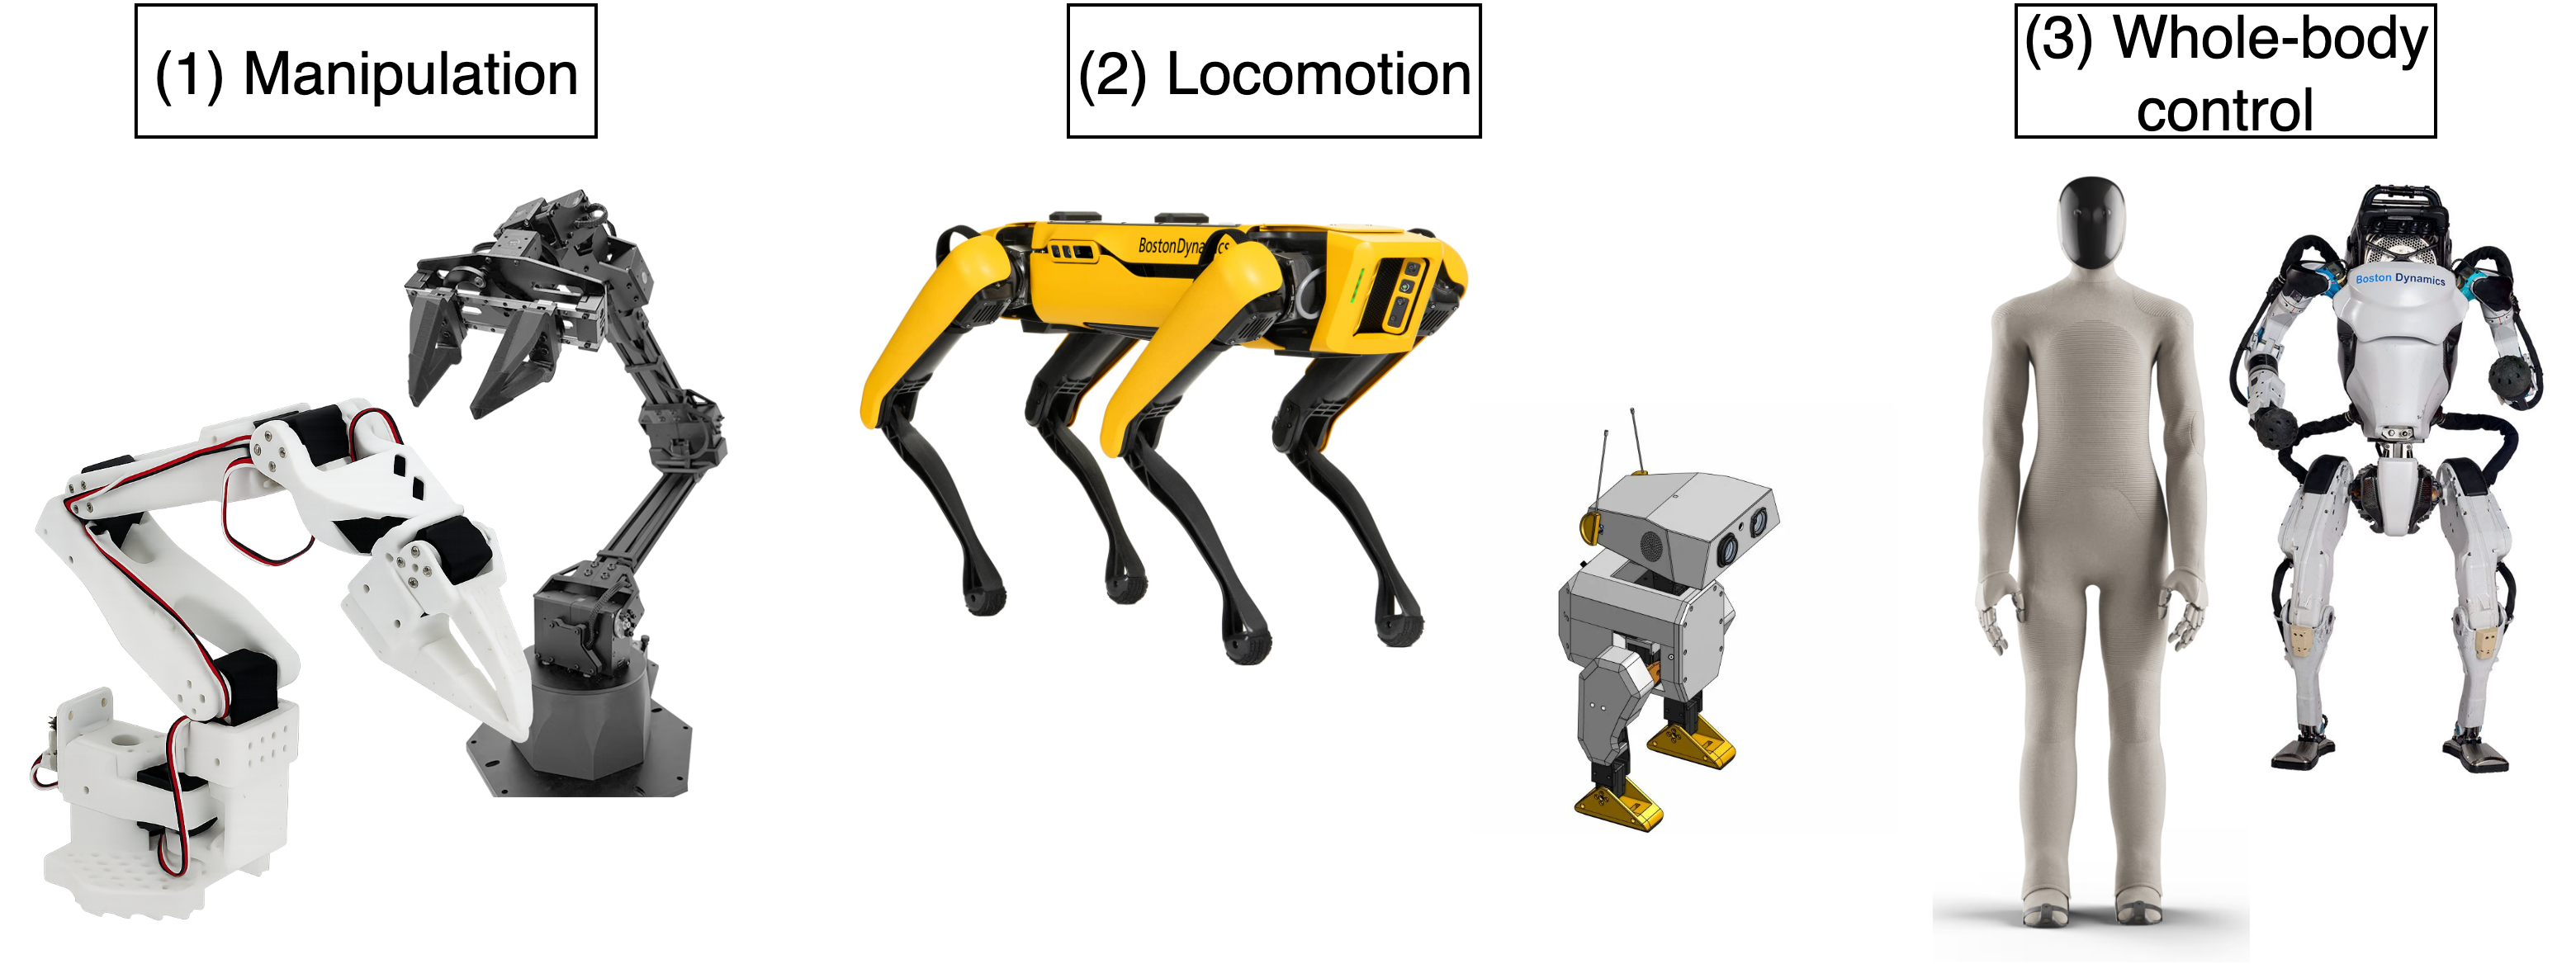
\includegraphics[width=0.7\linewidth]{figures/ch2/ch2-platforms.png}
    \caption{Different kinds of motions are achieved with potentially very different robotic platforms. From left to right, top to bottom: ViperX, SO-100, Boston Dynamics' Spot, Open-Duck, 1X's NEO, Boston Dynamics' Atlas. This is an example list of robotic platforms and is (very) far from being exhaustive.}
    \label{fig:robotics-platforms-atlas}
\end{figure}

% Robotics atlas: moving through and modifying an environment (and combinations). That is, (1) locomotion (2) manipulation and (3) whole-body control
At its very core, robotics deals with producing motion via actuating joints connecting nearly entirely-rigid links.
A key distinction between focus areas in robotics is based on whether the generated motion modifies (1) the absolute state of the environment (via dexterity), (2) the relative state of the robot with respect to its environment (exercising mobility skills), or (3) a combination of the two (Figure~\ref{fig:robotics-platforms-atlas}).

Effects such as (1) are typically achieved \emph{through} the robot, i.e. generating motion to perform an action inducing a desirable modification, effectively \emph{manipulating} the environment (manipulation).
Motions like (2) may result in changes in the robot's physical location within its environment.
Generally, modifications to a robot's location within its environment may be considered instances of the general \emph{locomotion} problem, further specified as \emph{wheeled} or \emph{legged} locomotion based on whenever a robot makes use of wheels or leg(s) to move in the environment.
Lastly, an increased level of dynamism in the robot-environment interactions can be obtained combining (1) and (2), thus designing systems capable to interact with \emph{and} move within their environment.
This category is problems is typically termed \emph{whole-body control}, and is characterized by a typically much larger set of control variables compared to either locomotion or manipulation alone.

% Focus on learning-based approaches and manipulation
The traditional body of work developed since the very inception of robotics is increasingly more complemented by learning-based approaches.
ML has indeed proven particularly transformative across the entire robotics stack, first empowering planning-based techniques with improved state estimation used for traditional planning~\citep{tangPerceptionNavigationAutonomous2023} and then end-to-end replacing controllers, effectively yielding perception-to-action methods~\citep{koberReinforcementLearningRobotics}.
Work in producing robots capable of navigating a diverse set of terrains demonstrated the premise of both dynamics and learning-based approaches for locomotion~\citep{griffinWalkingStabilizationUsing2017,jiDribbleBotDynamicLegged2023,leeLearningQuadrupedalLocomotion2020,margolisRapidLocomotionReinforcement2022}, and recent works on whole-body control indicated the premise of learning-based approaches to generate rich motion on complex robots, including humanoids~\citep{zhangWoCoCoLearningWholeBody2024,nvidiaGR00TN1Open2025}.
Manipulation has also been widely studied, particularly considering its relevance for many impactful applications ranging from high-risk applications for humans~\citep{fujitaDevelopmentRobotsNuclear2020,alizadehComprehensiveSurveySpace2024,fujitaDevelopmentRobotsNuclear2020} to manufacturing~\citep{sannemanStateIndustrialRobotics2020}.
While explicit models have proven fundamental in achieving important milestones towards the development of modern robotics, recent works leveraging implicit models proved particularly promising in surpassing scalability and practical applicability challenges via learning~\citep{koberReinforcementLearningRobotics}.

\subsection{Example: Planar Manipulation}
% Full physical description by means of forward kinematics to generate movement
Robot manipulators typically consist of a series of links and joints, articulated in a chain finally connected to an \emph{end-effector}.
Links and joints are considered responsible for generating motion, while the end effector is instead used to perform specific actions at the target location (e.g., grasping/releasing objects via closing/opening a gripper end-effector, using a specialized tool like a screwdriver, etc.).

Recently, the development of low-cost manipulators like the Aloha~\citep{zhaoLearningFineGrainedBimanual2023} Aloha-2~\citep{aldacoALOHA2Enhanced} and SO-100/SO-101~\citep{knightStandardOpenSO100} platforms significantly lowered the barrier to entry to robotics, considering the increased accessibility of these robots compared to more traditional platforms like the Franka Emika Panda arm (Figure~\ref{fig:robotic-platforms-costs}).

\begin{figure}
    \centering
    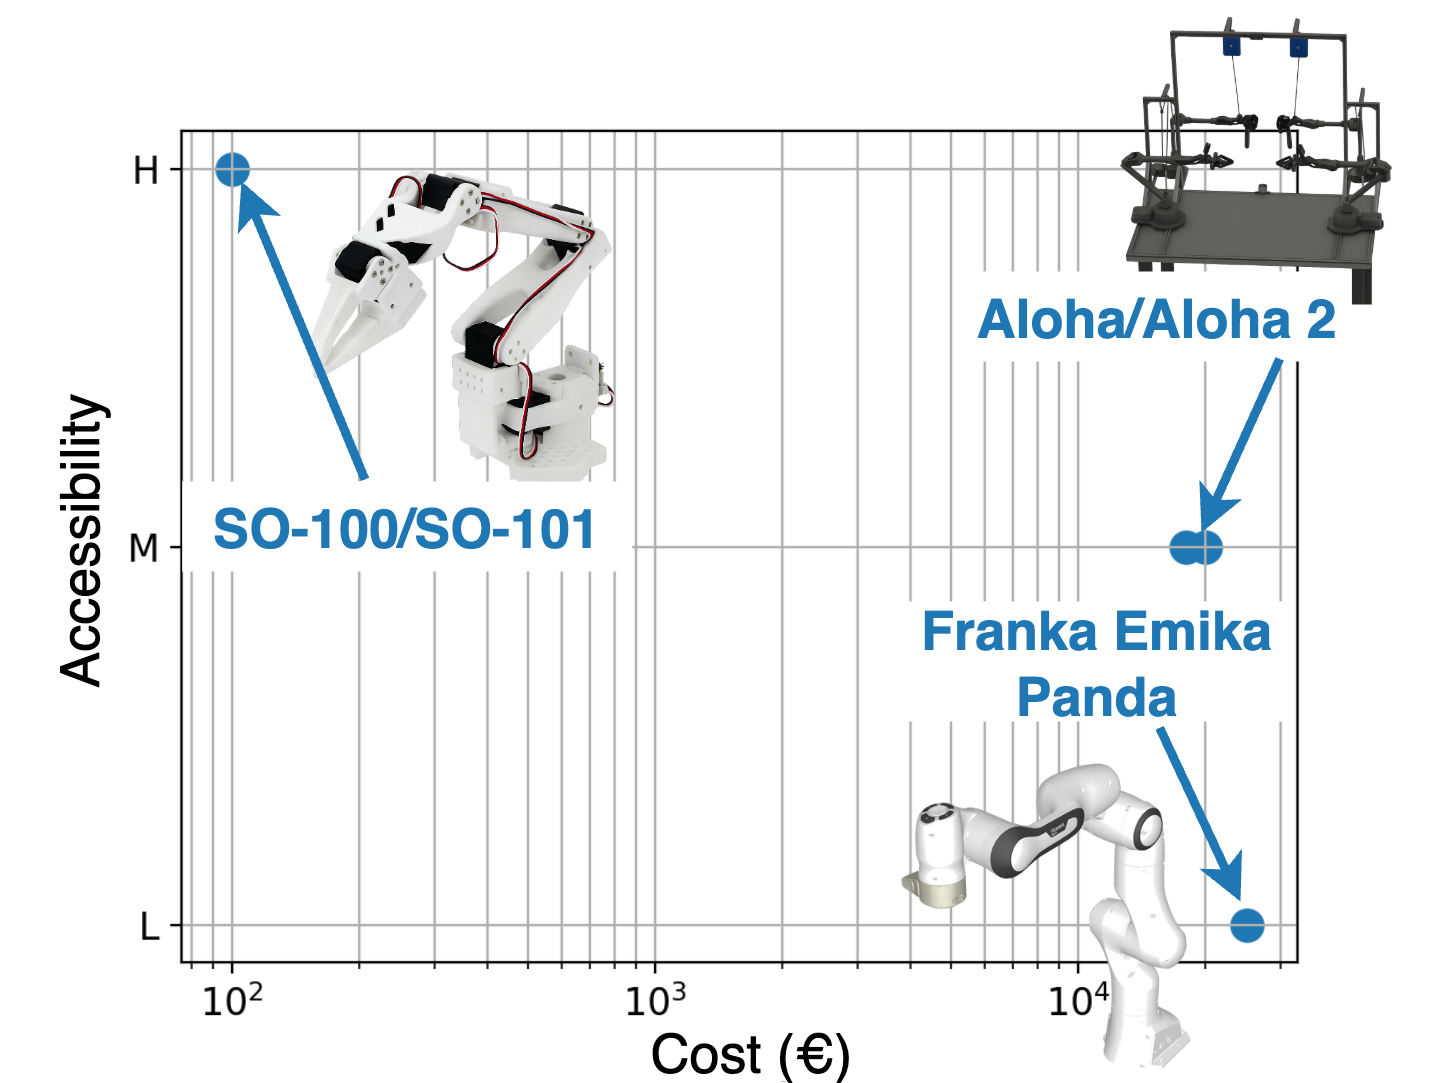
\includegraphics[width=0.4\linewidth]{figures/ch2/ch2-cost-accessibility.png}
    \caption{Cheaper, more accessible robots are starting to rival traditional platforms like the Panda arm platforms in adoption in resource-constrained scenarios. The SO-100, in particular, has a cost in the 100s of Euros, and can be entirely 3D-printed in hours, while the industrially-manufactured Panda arm costs tens of thousands of Euros and is not openly available.}
    \label{fig:robotic-platforms-costs}
\end{figure}

Deriving an intuition as per why learning-based approaches are gaining popularity in the robotics community requires briefly analyzing traditional approaches for manipulation, leveraging tools like forward and inverse kinematics (FK, IK) and control theory.
Providing a detailed overview of these methods falls (well) out of the scope of this tutorial, and we refer the reader to works including~\citet{sicilianoSpringerHandbookRobotics2016, lynchModernRoboticsMechanics2017, tedrakeRoboticManipulationPerception, tedrakeUnderactuatedRoboticsAlgorithms} for a much more comprehensive description of these techniques.
Here, we mostly wish to highlight the benefits of ML over these traditional techniques

\begin{figure}
    \centering
    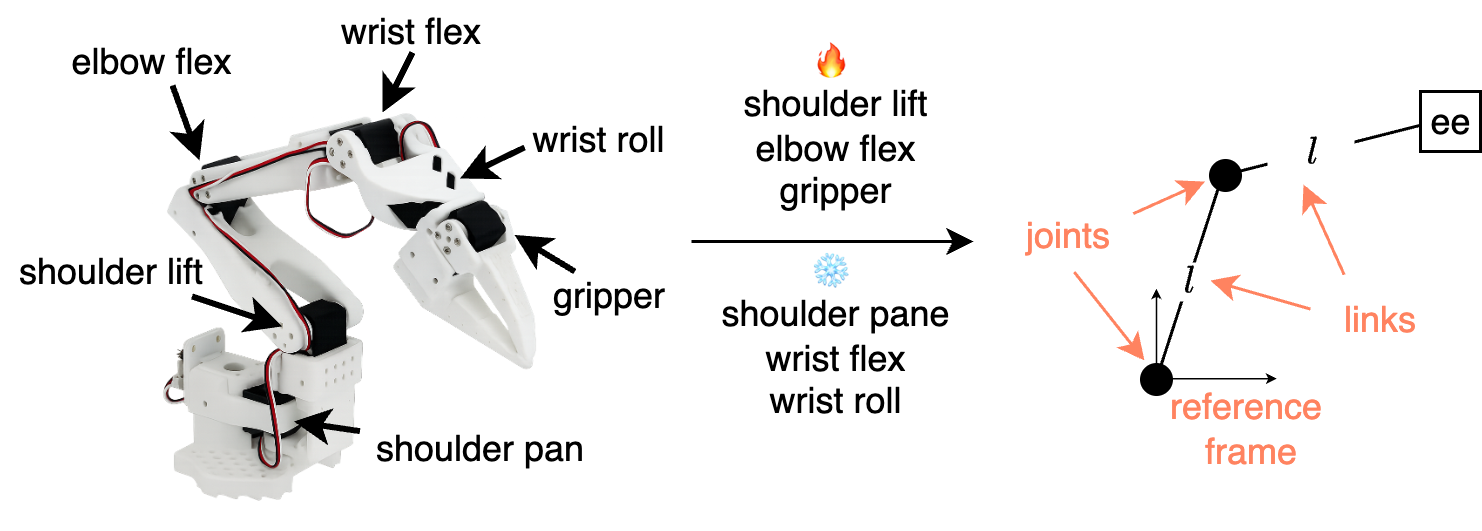
\includegraphics[width=0.7\linewidth]{figures/ch2/ch2-so100-to-planar-manipulator.png}
    \caption{The SO-100 arm is a 6-dof manipulator arm. Preventing some of its joints (shoulder pane, wrist flex and wrist roll) from actuating, it can be represented as a traditional 2-dof planar manipulator (the gripper joint in the end-effector is not considered towards the count of the degrees of freedom used to produce motion).}
    \label{fig:make-so100-planar-manipulator}
\end{figure}

Consider the (simple) case where a SO-100 is restrained from actuating (1) the shoulder pane and (2) the wrist flex and roll motors.
This effectively reduces the degrees of freedom of the SO-100 from the original 5+1 (5 joints + 1 gripper) to 2+1 (shoulder lift, elbow flex + gripper).
As the end-effector does not impact motion in this model, the SO-100 is effectively reduced to the planar manipulator robot presented in Figure~\ref{fig:make-so100-planar-manipulator}, where spheres represent actuators, and solid lines indicate links from the base of the SO-100 to the end-effector (\emph{ee}).

Further, let us make the simplifying assumption that actuators can produce rotations up to \( 2 \pi \) radians.
In practice, this is seldom the case due to movement obstructions caused by the robot body itself (for instance, the shoulder lift cannot produce counter-clockwise movement due to the presence of the robot's base used to secure the SO-100 to its support and host the robot bus), but we will introduce movement obstruction at a later stage.

All these simplifying assumptions leave us with the planar manipulator of Figure~\ref{fig:planar-manipulation-simple}, free of moving its end-effector by controlling the angles \( \theta_1 \) and \( \theta_2 \), jointly referred to as the robot's \emph{configuration}, and indicated with \( q = [\theta_1, \theta_2 ] \in [-\pi, +\pi]^2 \).
The axis attached to the joints indicate the associated reference frame, whereas circular arrows indicate the maximal feasible rotation allowed at each joint. 
In this tutorial, we do not cover topics related to spatial algebra, and we instead refer the reader to \citet[Chapter~2]{lynchModernRoboticsMechanics2017} and \citet[Chapter~3]{tedrakeRoboticManipulationPerception} for excellent explanations of the mechanics and theoretical foundations of producing motion on rigid bodies.

\newcommand{\panelheight}{3.2cm}  % keeping the following manipulators aligned requires images to be same height

\begin{figure}
    \centering
    \begin{subfigure}[t]{0.32\linewidth}
        \centering
        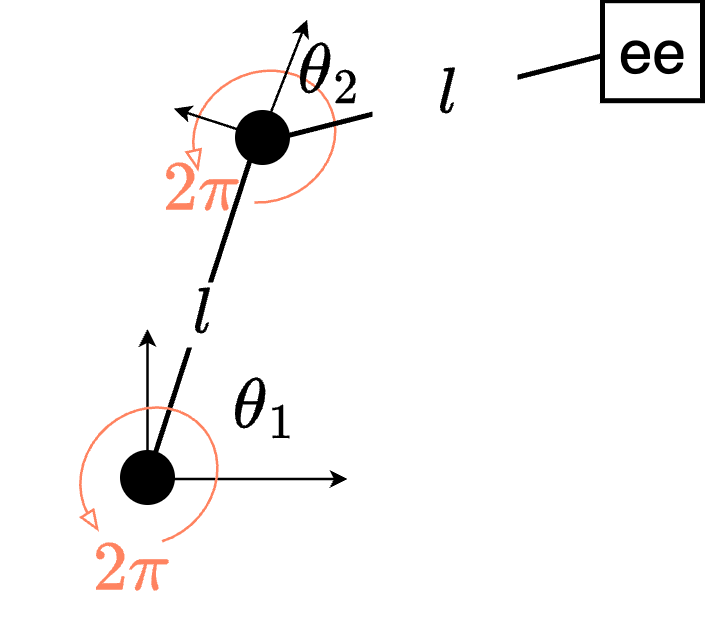
\includegraphics[width=\linewidth,height=\panelheight,keepaspectratio]{figures/ch2/ch2-planar-manipulator-free.png}
        \caption{Free to move}
        \label{fig:planar-manipulation-simple}
    \end{subfigure}\hfill
    \begin{subfigure}[t]{0.32\linewidth}
        \centering
        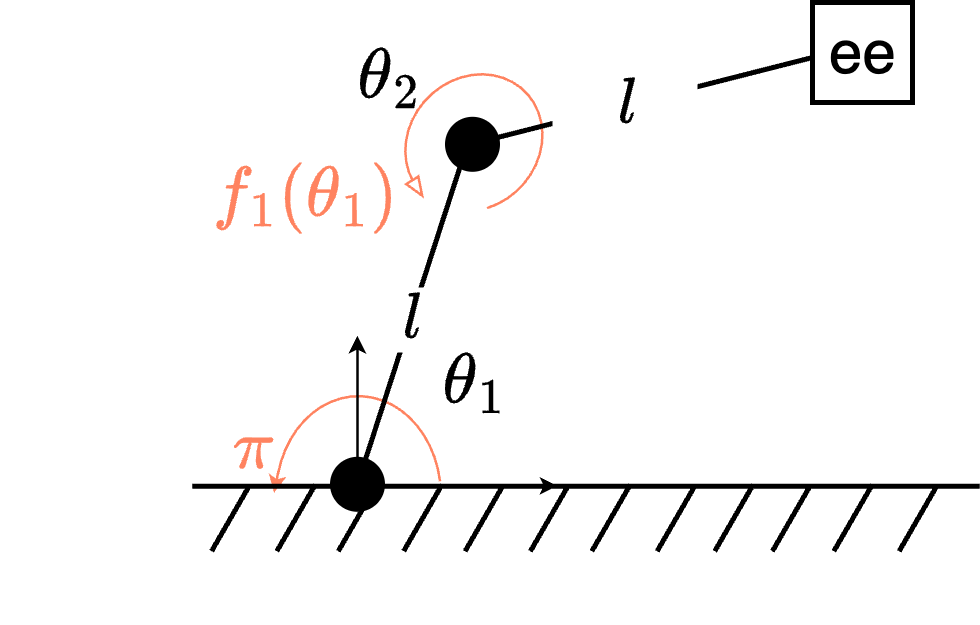
\includegraphics[width=\linewidth,height=\panelheight,keepaspectratio]{figures/ch2/ch2-planar-manipulator-floor.png}
        \caption{Constrained by the surface}
        \label{fig:planar-manipulator-floor}
    \end{subfigure}\hfill
    \begin{subfigure}[t]{0.32\linewidth}
        \centering
        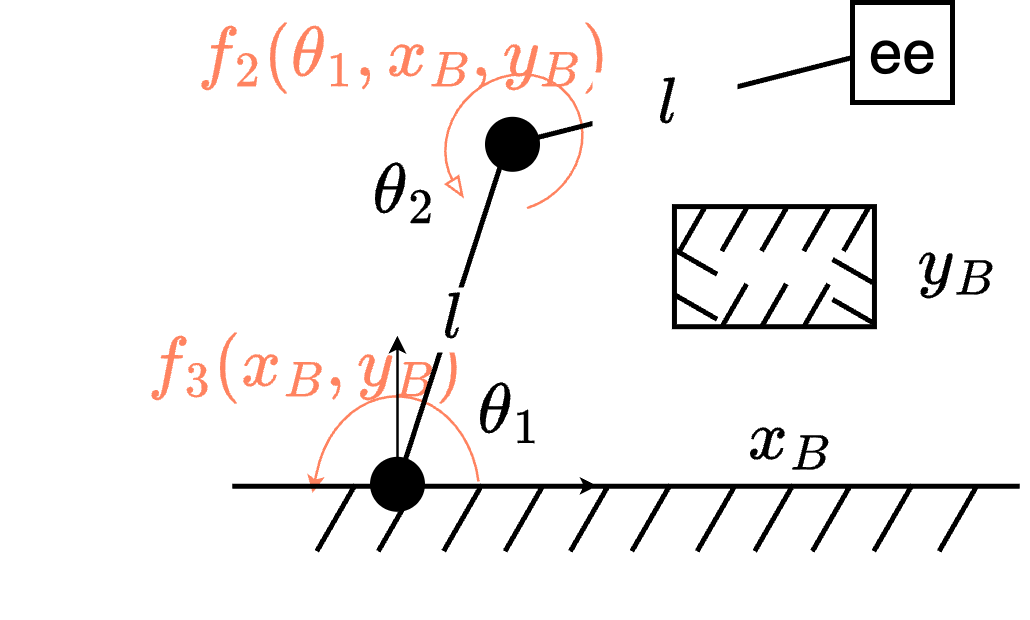
\includegraphics[width=\linewidth,height=\panelheight,keepaspectratio]{figures/ch2/ch2-planar-manipulator-floor-shelf.png}
        \caption{Constrained by surface and (fixed) obstacle}
        \label{fig:planar-manipulator-floor-shelf}
    \end{subfigure}
    \caption{Planar, 2-dof schematic representation of the SO-100 manipulator under diverse deployment settings. From left to right: completely free of moving; constrained by the presence of the surface; constrained by the surface and presence of obstacles. Circular arrows around each joint indicate the maximal rotation feasible at that joint.}
\end{figure}

Considering the (toy) example presented in Figure~\ref{fig:planar-manipulation-simple}, then we can analytically write the end-effector's position \( p \in \mathbb R^2 \) as a function of the robot's configuration, \( p = p(q), p: \mathcal Q \mapsto \mathbb R^2 \). 
In particular, we have:
\begin{equation*}
p(q) = 
\begin{pmatrix}
p_x(\theta_1, \theta_2) \\  
p_y(\theta_1, \theta_2)
\end{pmatrix}
=
\begin{pmatrix}
l \cos(\theta_1) + l \cos(\theta_1 + \theta_2) \\
l \sin(\theta_1) + l \sin(\theta_1 + \theta_2)
\end{pmatrix}
\in S^{n=2}_{l_1+l_2} = \{ p(q) \in \mathbb R^2: \Vert p(q) \Vert_2^2 \leq (2l)^2, \ \forall q \in \mathcal Q \}
\end{equation*}

Deriving the end-effector's \emph{pose} in some \(m\)-dimensional space \( \vec{p} \in \mathcal{P} \subset \mathbb{R}^{m} \) (position and orientation) starting from the configuration \( \q \in \mathcal Q \subset \mathbb R^n \) of a \( n \)-joints robot is referred to as \emph{forward kinematics} (FK), whereas identifying the configuration corresponding to any given target pose is termed \emph{inverse kinematics} (IK).
In that, FK is used to map a robot configuration into the corresponding end-effector pose, whereas IK is used to reconstruct the configuration(s) given an end-effector pose.

In the simplified case here considered (for which \( \vec{p} \equiv p \), as the orientation of the end-effector is disregarded for simplicity), one can solve the problem of controlling the end-effector's location to reach a goal position \( p^* \) by solving analytically for \( q: p(q) = f_{\FK}(q) = p^*\).
However, in the general case, one might not be able to solve this problem analytically, and can typically resort to iterative optimization methods comparing candidate solutions using a loss function (in the simplest case, \( \Vert p(q) - p^* \Vert_2^2 \) is a natural candidate), yielding:

\begin{align}
\min_{q \in \mathcal Q} \Vert p(q) - p^* \Vert_2^2
\label{eq:ik_problem}
\end{align}

Analytical solutions are even less appealing when one considers the presence of obstacles in the robot's workspace, resulting in constraints on the possible values of \( q \in \mathcal Q \subseteq [-\pi, +\pi]^n \subset \mathbb R^n \) in the general case of \(n\)-links robots.

For instance, the robot in Figure~\ref{fig:planar-manipulator-floor} is (very naturally) obstacled by the presence of the surface upon which it rests: \( \theta_1 \) can now exclusively vary within \([0,  \pi] \), while possible variations in \( \theta_2 \) depend on \( \theta_1 \) (when \( \theta_1 \to 0 \) or \( \theta_1 \to \pi \), further downwards movements are restricted).
Even for a simplified kinematic model, developing techniques to solve~\ref{eq:ik_problem} is in general non-trivial in the presence of constraints, particularly considering that the feasible set of solutions \( \mathcal Q \) may change across problems.
Figure~\ref{fig:planar-manipulator-floor-shelf} provides an example of how the environment influences the feasible set considered, with a new set of constraints deriving from the position of a new obstacle.

Further, IK---solving \ref{eq:ik_problem} for a feasible \( q \)---only proves useful in determining information regarding the robot's configuration in the goal pose, and crucially does not provide information on the \emph{trajectory} to follow over time to reach a target pose.
Expert-defined trajectories obviate to this problem providing a length-\(K\) succession of goal poses \( \tau_K = [p^*_0, p^*_1, \dots p^*_K] \) for tracking.
In practice, trajectories can also be obtained automatically through \emph{motion planning} algorithms, thus avoiding expensive trajectory definition from human experts.
However, tracking \( \tau_K \) via IK can prove prohibitively expensive, as tracking would require \( K \) resolutions of \ref{eq:ik_problem} (one for each target pose).
\emph{Differential} inverse kinematics (diff-IK) complements IK by enabling adaptive trajectory tracking. 
Let \( J(q) \) denote the Jacobian matrix of (partial) derivatives of the FK-function \( f_\FK: \mathcal Q \mapsto \mathcal P \), such that \( J(q) = \frac{\partial f_{FK}(q)}{\partial q } \).
Then, one can apply the chain rule to any \( p(q) = f_{\FK}(q) \), deriving \( \dot p = J(q) \dot q \), and thus finally relating variations in the robot configurations to variations in pose, thereby providing a platform for control.

Given a desired end-effector trajectory \( \targetvel(t) \) (1) indicating ancor regions in space  and (2) how much time to spend in each region, diff-IK finds \( \dot q(t) \) solving for joints' \emph{velocities} instead of \emph{configurations},
\begin{align}
\dot q(t) = \arg\min_\nu \; \lVert J(q(t)) \nu - \targetvel (t) \rVert_2^2
\label{eq:reg_ik_velocity}
\end{align}

Unlike~\ref{eq:ik_problem}, solving for \( \dot q \) is much less dependent on the environment (typically, variations in velocity are constrained by physical limits on the actuators represented with box-like constraints in \ref{eq:reg_ik_velocity}).
Conveniently, \ref{eq:reg_ik_velocity} also often admits the closed-form solution \( \dot q = J(q)^+ \targetvel \), where \( J^+(q) \) denotes the Moore-Penrose pseudo-inverse of \( J(q) \).
Finally, discrete-time joint configurations \( q \) can be reconstructed from joint velocities \( \dot q \) using forward-integration on the continuous-time joint velocity , \( q_{t+1} = q_t + \Delta t\,\dot q_t \) for a given \( \Delta t \), resulting in tracking via diff-IK.

Following trajectories with diff-IK is a valid option in well-controlled and static environments (e.g., industrial manipulators in controlled manufacturing settings), and relies on the ability to define a set of target velocities to track \( [\targetvel_0, \targetvel_1, \dots, \targetvel_k ] \)---an error-prone task largely carried out by human experts.
Furthermore, diff-IK relies on the ability to (1) access \( J(q) \, \forall q \in \mathcal Q \) and (2) compute its pseudo-inverse at every iteration of a given control cycle---a challenging assumption in highly dynamical settings, or for complex kinematic chains, or nonlinear dynamics.

\subsubsection{Adding Feedback Loops}
While very effective when a goal trajectory has been well specified, the performance of diff-IK can degrade significantly in the presence of modeling/tracking errors, or in the presence of non-modeled dynamics in the environment.

\begin{wrapfigure}[12]{r}{0.3\textwidth}
    \vspace{-\intextsep}
    \centering
    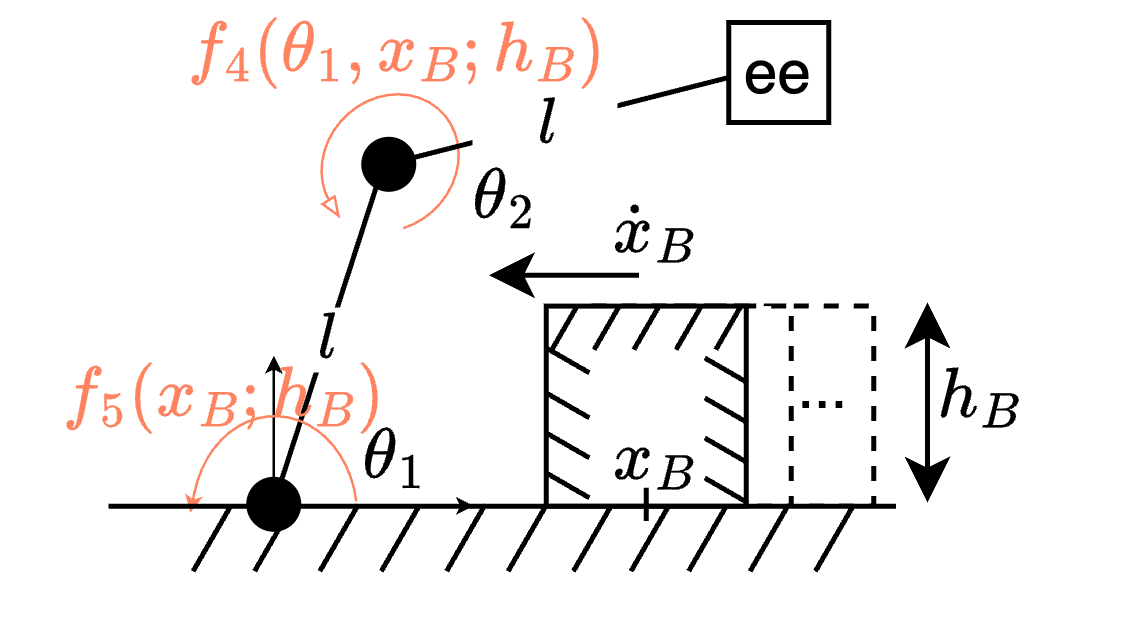
\includegraphics[width=\linewidth]{figures/ch2/ch2-planar-manipulator-floor-box.png}
    \caption{Planar manipulator robot in the presence of a moving obstacle.}
    \label{fig:planar-manipulator-box-velocity}
\end{wrapfigure}

One such case is presented in Figure~\ref{fig:planar-manipulator-box-velocity}, where another rigid body other than the manipulator is moving in the environment along the horizontal axis, with velocity \( \dot x_B \).
Accounting analytically for the presence of this disturbance---for instance, to prevent the midpoint of \( l_1 \) from ever colliding with the object---requires access to \( \dot x_B \) at least, to derive the equation characterizing the motion of the environment.

Less predictable disturbances however (e.g., \( \dot x_B \leftarrow \dot x_B + \eps, \eps \sim N(0,1) \)) may prove challenging to model analytically, and one could attain the same result of preventing link-object collision by adding a condition on the distance between the midpoint of \( l_1 \) and \( x_B \), enforced through a feedback loop on the position of the robot and object at each control cycle.

To mitigate the effect of modeling errors, sensing noise and other disturbances, classical pipelines indeed do augment diff-IK with feedback control looping back quantities of interest.
In practice, following a trajectory with a closed feedback loop might consist in backwarding the error between the target and measured pose, \( \Delta p = \targetpos - p(q) \), hereby modifying the control applied to \( \dot q = J(q)^+ (\targetvel + k_p \Delta p ) \), with \( k_p \) defined as the (proportional) gain.

More advanced techniques for control consisting in feedback linearization, PID control, Linear Quatratic Regulator (LQR) or Model-Predictive Control (MPC) can be employed to stabilize tracking and reject moderate perturbations (\citep[Chapter~8]{sicilianoSpringerHandbookRobotics2016} for in-detail explanation of these concepts, or \citep[Chapter~8]{tedrakeRoboticManipulationPerception} for a simple, intuitive example in the case of a point-mass system).
Nonetheless, feedback control presents its challenges as well: tuning gains remains laborious and system-specific. 
In particular, manipulation tasks present intermittent contacts inducing hybrid dynamics (mode switches) and discontinuities in the effective Jacobian, challenging the stability guarantees of the controller and thus often necessitating rather conservative gains and substantial hand-tuning.

We point the interested reader to~\citet[Chapter~2,7,8]{sicilianoSpringerHandbookRobotics2016}, \citet[Chapter~6,11]{lynchModernRoboticsMechanics2017}, and~\citet[Chapter~3,8]{tedrakeRoboticManipulationPerception} for extended coverage of FK, IK, diff-IK and control for (diff-)IK.

\subsection{Limitations of Dynamics-based Robotics}
Despite the last 60+ years of robotics research, autonomous robots are still largely incapable of performing tasks at human-level performance in the physical world generalizing across (1) robot embodiments (different manipulators, different locomotion platforms, etc.) and (2) tasks (tying shoe-laces, manipulating a diverse set of objects).
While essential in the early development of robotics, the aforementioned methods require significant human expertise to be used in practice, and are typically specific to a particular applicative problem.

\begin{figure}
    \centering
    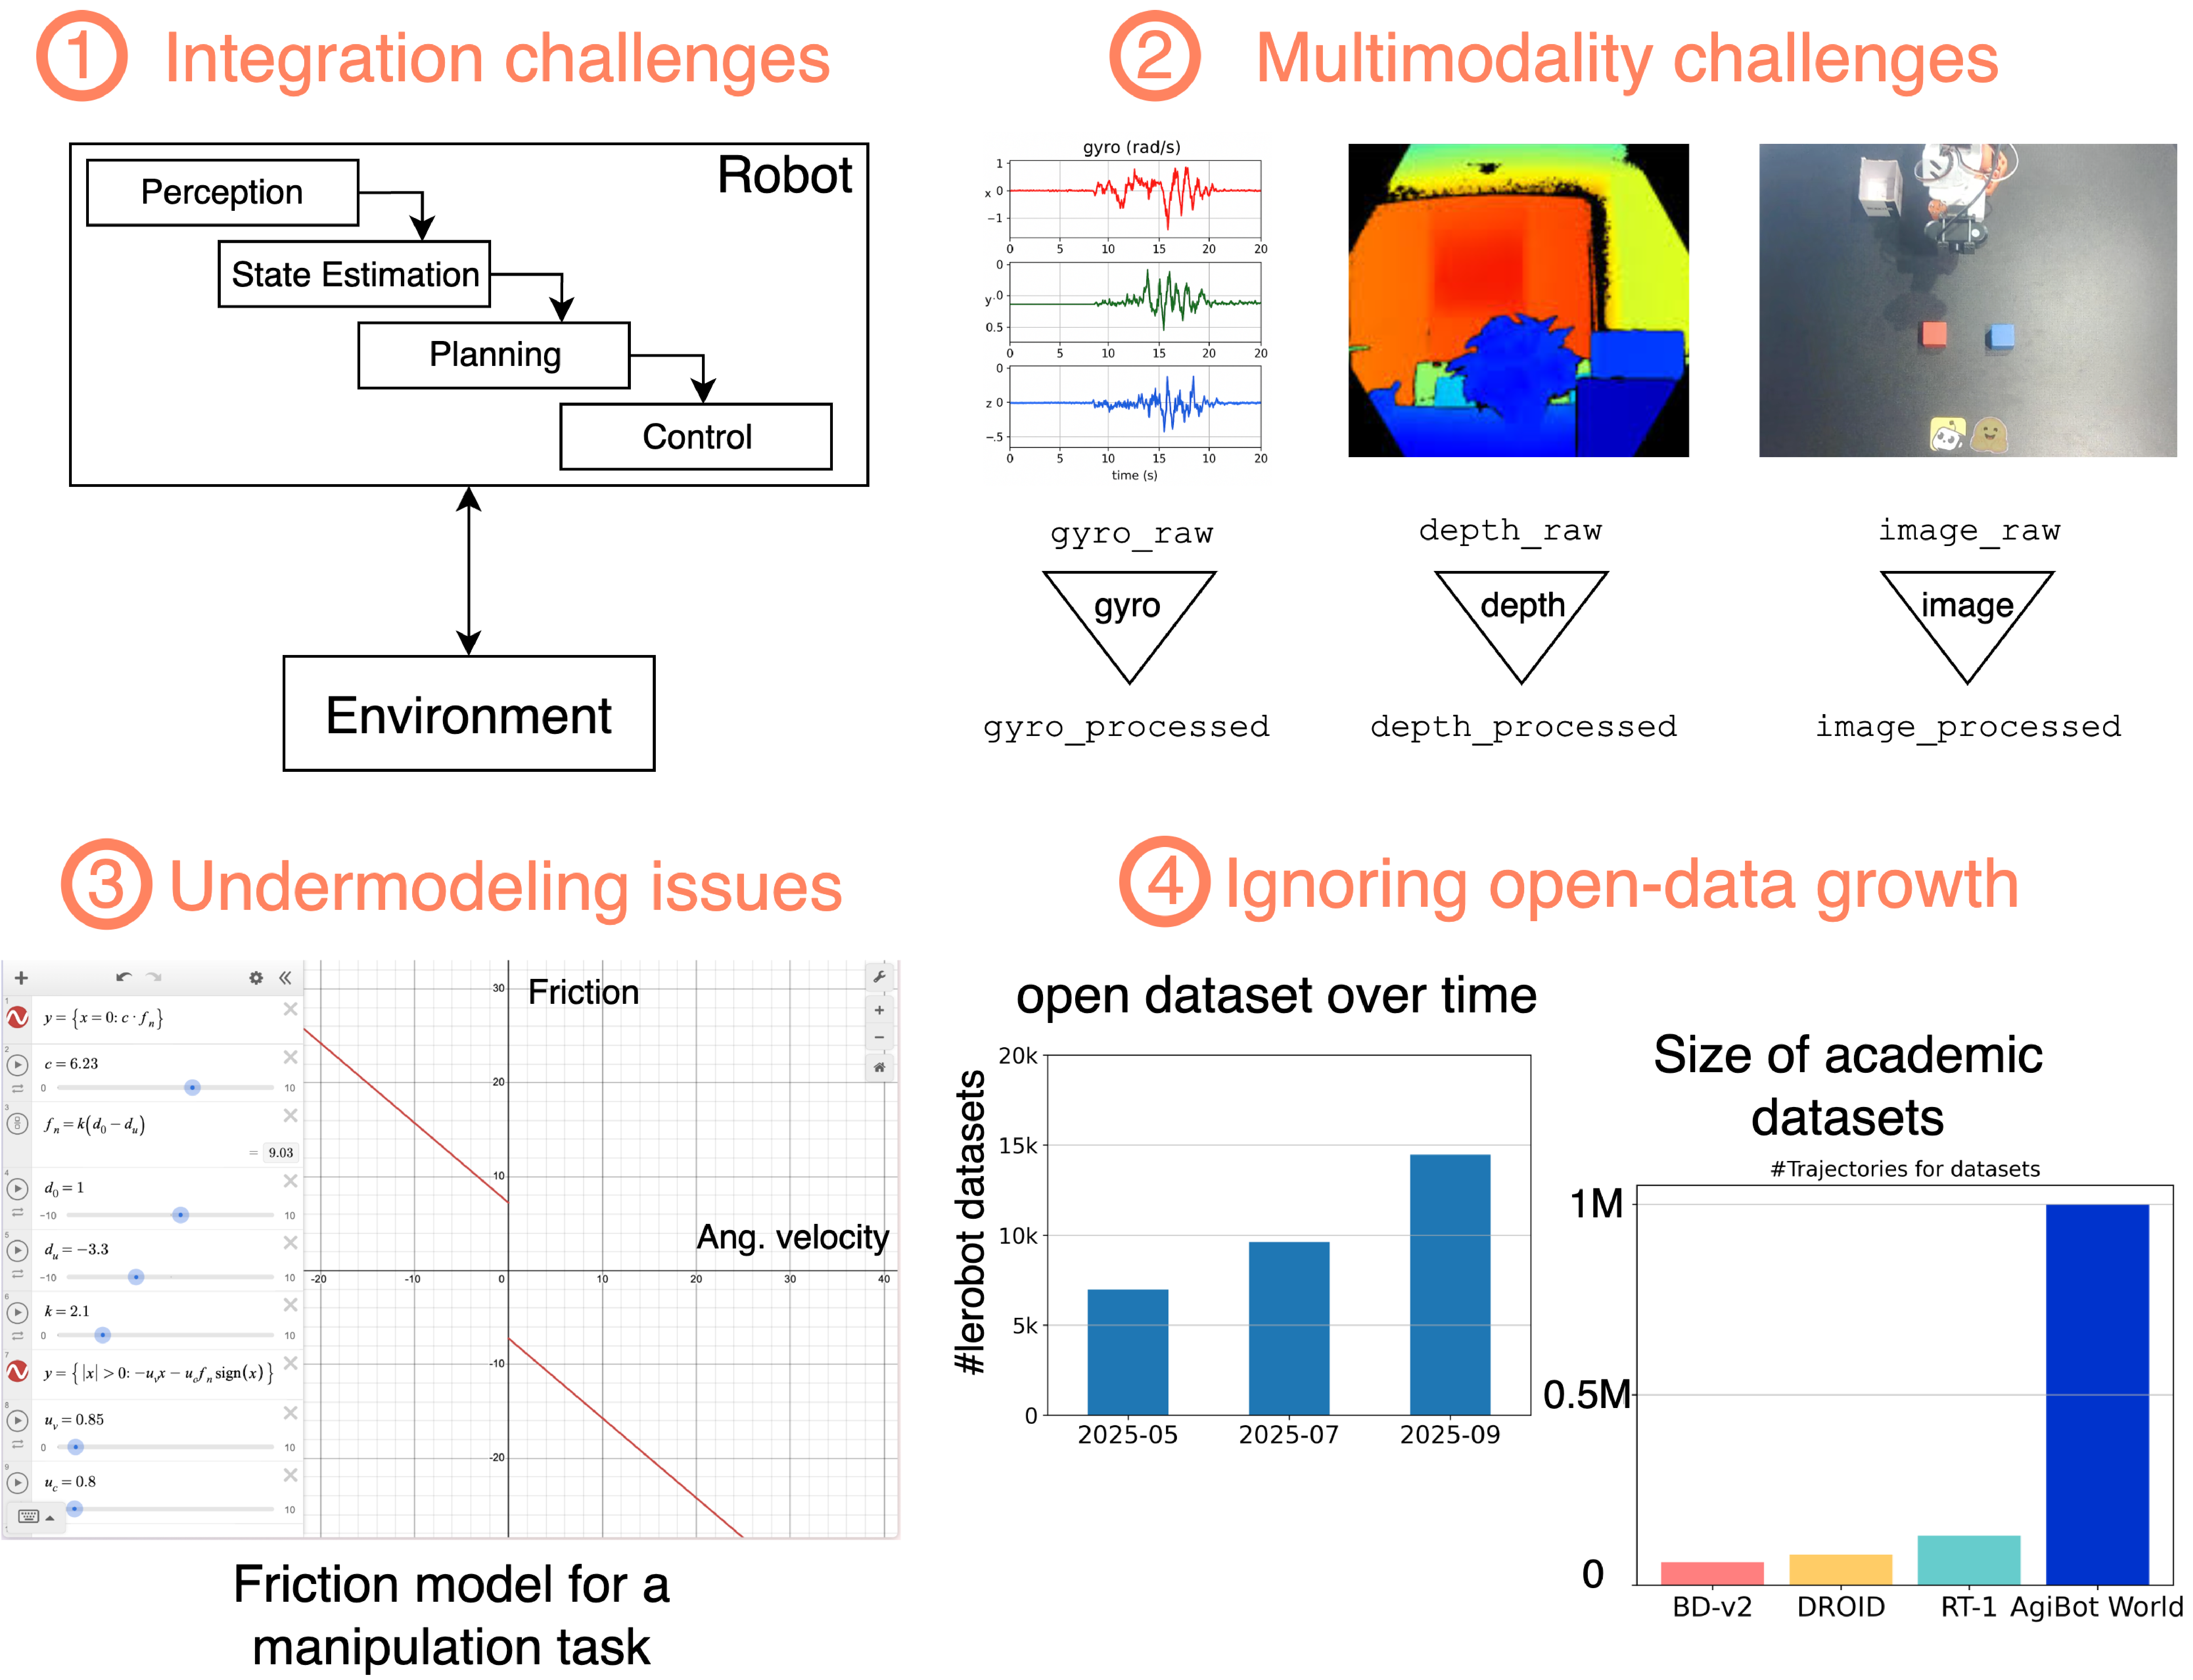
\includegraphics[width=0.9\linewidth]{figures/ch2/ch2-classical-limitations.png}
    \caption{Dynamics-based approaches to robotics suffer from several limitations: (1) orchestrating multiple components poses integration challenges; (2) the need to develop custom processing pipelines for the sensing modalities and tasks considered hinders scalability; (3) simplified analytical models of physical phenomena (here friction at the gripper; credits to~\citet{antonovaReinforcementLearningPivoting2017}) limit real-world performance. Lastly, (4) dynamics-based methods overlook trends in the availability and growth of robotics data.}
    \label{fig:classical-limitations}
\end{figure}

Dynamics-based robotics pipelines have historically been \highlight{developed sequentially, engineering the different blocks} now within most architectures for specific purposes.
That is, sensing, state estimation, mapping, planning, (diff-)IK, and low-level control have been traditionally developed as distinct modules with fixed interfaces.
Pipelining these specific modules proved error-prone, and brittleness emerges---alongside error compounding---whenever changes incur (e.g., changes in lighting for sensing, occlusion/failure of sensors, control failures).
Adapting such a stack to new tasks or robotic platforms often entails re-specifying objectives, constraints, and heuristics at multiple stages, incurring significant engineering overhead.

Moreover, classical planners operate on compact, assumed-sufficient state representations; extending them to reason directly over raw, heterogeneous and noisy data streams is non-trivial.
This results in a \highlight{limited scalability to multimodal data and multitask settings}, as incorporating high-dimensional perceptual inputs (RGB, depth, tactile, audio) traditionally required extensive engineering efforts to extract meaningful features for control. 
Also, the large number of tasks, coupled with the adoption of \emph{per-task} planners, goal parameterizations, and safety constraints, results in an explosion in design and validation options, with little opportunity to reuse solutions across tasks.

Setting aside integration and scalability challenges: developing accurate modeling of contact, friction, and compliance for complicated remains difficult.
Rigid-body approximations are often insufficient in the presence of deformable objects, and \highlight{relying on approximated models hinders real-world applicability} of the methods developed.
In the case of complex, time-dependent and/or non-linear dynamics, even moderate mismatches in parameters, unmodeled evolutions, or grasp-induced couplings can qualitatively affect the observed dynamics.

Lastly, dynamics-based methods (naturally) overlook the rather recent \highlight{increase in availability of openly-available robotics datasets}. 
The curation of academic datasets by large centralized groups of human experts in robotics~\citep{OpenXEmbodimentRobotic,DROIDLargeScaleIntheWild,agibot-world-contributorsAgiBotWorldColosseo2025} is now increasingly complemented by a \highlight{growing number of robotics datasets contributed in a decentralized fashion} by individuals with varied expertises.
If not tangentially, dynamics-based approaches are not posed to maximally benefit from this trend, which holds the premise of allowing generalization in the space of tasks and embodiments, like data was the cornerstone for advancements in vision~\citep{alayracFlamingoVisualLanguage2022} and natural-language understanding~\citep{brownLanguageModelsAre2020}.

Taken together, these limitations (Figure~\ref{fig:classical-limitations}) motivate the exploration of learning-based approaches that can (1) integrate perception and control more tightly, (2) adapt across tasks and embodiments with reduced expert modeling interventions and (3) scale gracefully in performance as more robotics data becomes available.